\documentclass[a4paper, 11pt]{article}
\title{Project: Automaten}
\author{Bas Van Assche, Tom Martens}
\usepackage[utf8]{inputenc}
\usepackage{hyperref}						%snelkoppeling in inhoudstafel
\usepackage{float}
\usepackage{graphicx} 						%foto's
\usepackage[usenames,dvipsnames]{color} 	%kleuren van woorden
\usepackage{url}
\hypersetup{
	colorlinks,
	citecolor=black,
	filecolor=black,
	linkcolor=black,
	urlcolor=black
}

\usepackage[dutch]{babel}
\usepackage[parfill]{parskip}
\usepackage[plain]{fancyref}
\usepackage[dvipsnames]{xcolor}
\usepackage{xspace}
\usepackage{amsmath}
\usepackage{amssymb}
\usepackage{mathtools}

\setlength{\textwidth}{0.75\paperwidth}
\setlength{\oddsidemargin}{0cm}
\setlength{\marginparwidth}{0cm}
\setlength{\marginparsep}{0cm}
\setlength{\voffset}{-2cm}
\setlength{\textheight}{700pt}


%%%%%%%%%%%%%%%%%%%%%%%%%%%%%%%

%%%%%%%%%%%%%%%%%%%%%%%%%%%%%%%


%header and footer
\usepackage{fancyhdr}
\pagestyle{fancy}
\lhead{Project: Automaten}
%header and footer

\begin{document}
	\maketitle
	\tableofcontents
	\newpage
	\section{Inleiding}
		Dit is een kort verlag waarin we bespreken hoe we alles hebben geïmplementeerd, wie welke onderdelen uitgevoerd heeft en welke problemen we zijn tegengekomen en hoe we die hebben aangepakt.
	
	\section{Structuur implementatie en beschrijving klassen}
		\textbf{Class Automaton:}
		Dit is de implementatie van de automaat zelf. Op deze automaat kan een intersectie met een andere automaat uitgevoerd worden en het kortste geaccepteerde pad of het kortste niet geaccepteerde pad kan gezocht worden. Een automaat wordt voorgesteld door een verzameling van States, finishstates en een startstate. Met de functies addEdge, addFinish en setStart wordt de automaat opgebouwd.
		
		\textbf{Class State:}
		Een State heeft een label en een lijst met Edges die vertrekken vanuit de state. Met de functie getEdgesStartingFromHere() kan men de lijst met Edges opvragen.
		
		\textbf{Class Edge:}
		Deze klasse stelt een edge voor uit de automaat met een start-state, een finish-state en een symbool.
		
		\textbf{Class AutomatonParser:}
		Deze klasse kan een automaat inlezen vanuit een bestand en die automaat kan dan ook opgevraagd worden.
		
		\textbf{Class Level0:}
		Bij level 0 wordt het kortste pad van een automaat gegeven en indien er geen pad is wordt er “null” gegeven.
		
		\textbf{Class Level1:}
		Bij level 1 wordt het kortste pad van een automaat gegeven waarbij er 2 schatten gevonden zijn. De tweede voorwaarde is dat er een sleutel nodig is om door een deur te gaan. Een de laatste voorwaarde is dat men onmiddellijk in de rivier moet springen wanneer men langs de draak gaat en geen zwaard heeft. De nodige automaten wordt met de AutomatonParser klasse ingelezen vanuit een file.
		
		\textbf{Class Level2:}
		Bij level 2 is gelijkend aan level 1. Het verschil is dat mem alle reeds gevonden schatten verliest wanneer men door een boog gaat. Ook hier worden de nodige automaten ingelezen vanuit een file.
		
		\section{Taakverdeling}
		De implementatie van de automaat is door Bas geïmplementeerd en de levels en de main klasse zijn door Tom geïmplementeerd.
		
		\section{Implementatie van levels}
		De levels zijn ontworpen om zo weinig mogelijk nodes te bevatten. Level 1 en 2 bestaan uit 3 verschillende automaten die vermenigvuldigd worden. 
		
		Dit zijn de verschillende automaten die we gebruikt hebben voor de levels:
		
		\begin{figure}[H]
			\centering
			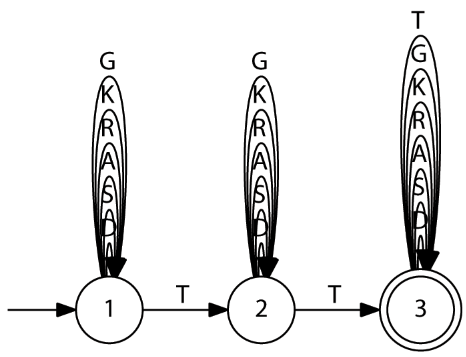
\includegraphics[width=0.4\linewidth]{2schatten}
			\caption{Minstens twee schatten vinden.}
			\label{fig:2schatten}
		\end{figure}
		
		In \fref{fig:2schatten} zien we de automaat die de voorwaarde oplegt twee schatten te vinden. 
	
		
		\begin{figure}[H]
			\centering
			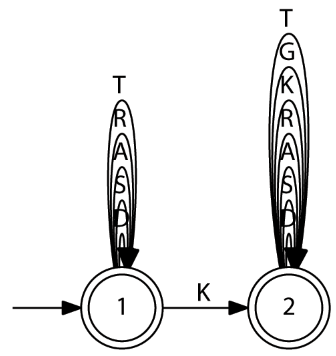
\includegraphics[width=0.3\linewidth]{sleutel}
			\caption{Sleutel vinden voor je door een deur kan.}
			\label{fig:sleutel}
		\end{figure}
	
		In \fref{fig:sleutel} zien we de automaat waarbij men een sleutel moet vinden voor het openen van en deur. Dus voor het vinden van de sleutel kan alles gedaan worden behalve door een deur gaan. Na het vinden van de sleutel kunnen wel alle tekens worden gelezen.	
		
		\begin{figure}[H]
			\centering
			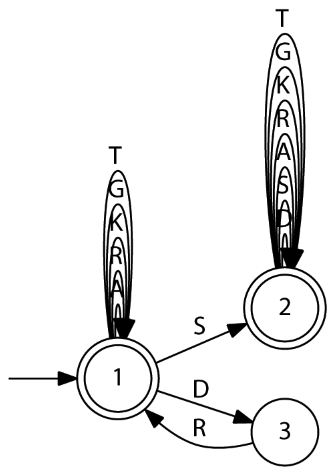
\includegraphics[width=0.3\linewidth]{draak}
			\caption{Na het passeren van een draak in het water springen als je geen zwaard hebt.}
			\label{fig:draak}
		\end{figure}
	
		In \fref{fig:draak} zien we de automaat die beschrijft wat er moet gebeuren bij de draak. De automaat begin in een accept toestand. Wanneer men daarna een draak tegenkomt zal men direct via een rivier moeten gaan om terug een een accept toestand te komen. Na het vinden van een zwaard, wordt deze beperking niet meer opgelegd.
			
		
		\begin{figure}[H]
			\centering
			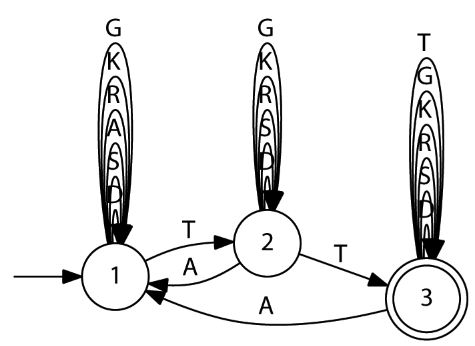
\includegraphics[width=0.4\linewidth]{boog}
			\caption{Bij het passeren van een boog speel je alle schatten kwijt.}
			\label{fig:boog}
		\end{figure}
		
		Als men in level 2 een boog passeert moet men alle schatten verliezen. We hebben dit gecombineerd met het zoeken van de twee schatten zoals in \fref{fig:boog} te zien is. We geraken enkel in een eindtoestand door twee of meer schatten te bezitten. Telkens als we een boog passeren gaan we terug naar de begintoestand. Dit komt overeen met het verliezen van de schatten.
	
	\section{Problemen}
		Na het implementeren van de levels kwamen tot de conclusie dat bij adventure 1 in level 2 we niet tot een resultaat kwamen. We kwamen tot de conclusie dat er enorm veel berekend moest worden omdat de automaat na intersectie meer dan 500 nodes groot is. We hebben geprobeerd dit op te lossen door de deelautomaten kleiner te maken. Maar het algoritme versnelde niet genoeg om in redelijke tijd een resultaat te krijgen. We hebben dit probleem opgelost door de implementatie van $getShortestExample()$ aan te passen. Wanneer men een node voor de tweede keer tegenkomt weten we dat het huidige pad niet tot een kortste oplossing kan komen. Wanneer men een node meermaals tegenkomt zit er een loop in het pad en bestaat er dus een korter pad dat deze loop niet bevat.
	
	
	
	
	
	
	
	
	
	
	
\end{document}